\documentclass[10.5pt]{article}
\usepackage[margin=1.1in]{geometry}
\usepackage[utf8]{inputenc}
\usepackage{ amssymb }
\usepackage{amsmath}
\usepackage{mdframed}
\usepackage{minted}
\surroundwithmdframed[linewidth = 1pt]{minted}
\usepackage{parskip}
\usepackage{graphicx}
\usepackage{float}
\usepackage{tikz}
\usepackage{fancyhdr}
\setlength{\headheight}{3cm}
\pagestyle{fancy}
\renewcommand{\headrulewidth}{0pt}


\lhead{
\begin{minipage}{2.5cm}
\begin{figure}[H]
\includegraphics[width=2.5cm]{oie_logo.png}
\end{figure}
\end{minipage} 
\begin{minipage}{8cm}
\textbf{XXV Olimpiada Inform\'atica Espa\~nola}\\
Pruebas de sistema\\
\texttt{histograma}
\end{minipage}
}

\begin{document}



\section*{Histograma}

Hay una imagen de $n \times n$ p\'ixeles que representa un histograma, es decir, un gr\'afico de columnas en la que hay $n$ columnas que est\'an marcadas con p\'ixeles negros hasta una cierta altura y con p\'ixeles blancos m\'as arriba.

\begin{center}
\begin{tikzpicture}
\draw[step=1cm,gray,very thin] (0,0) grid (6,6);
\fill[black] (0,0) rectangle (1,3);
\fill[black] (1,0) rectangle (2,1);
\fill[black] (3,0) rectangle (4,5);
\fill[black] (4,0) rectangle (5,2);
\fill[black] (5,0) rectangle (6,3);
\end{tikzpicture}
\end{center}

Por ejemplo, esta imagen $6 \times 6$ representa un histograma con alturas $3, 1, 0, 5, 2, 3$. La altura m\'axima de las columnas en este histograma es $5$.

El objetivo es encontrar la altura m\'axima de las columnas del histograma consultando como m\'aximo $10\,000$ p\'ixeles de la imagen.

\subsection*{Entrada y salida}

\textbf{Este es un problema interactivo}. Debes refrescar la salida cada vez que imprimas datos (\texttt{cout << endl} o \texttt{cout << flush} en C++, \texttt{System.out.flush()} en Java, \texttt{stdout.flush()} en Python).

La primera l\'inea de la entrada contiene un entero $n$, la dimensi\'on de la imagen. Debes leer este valor antes de hacer ninguna pregunta.

Para consultar un p\'ixel debes escribir una l\'inea con el formato \verb#? x y#, donde $x, y$ son las coordenadas del p\'ixel que quieres consultar ($0 \leq x, y \leq n-1$, $x$ es la coordenada horizontal en el sentido de izquierda a derecha e $y$ es la coordenada vertical en el sentido de abajo a arriba ($(0, 0)$ es la esquina inferior izquierda y $(n-1, n-1)$ la esquina superior derecha)). A continuaci\'on debes leer una l\'inea con el resultado, que ser\'a un \verb#1# si el p\'ixel es negro o un \verb#0# si es blanco. En caso de que hayas superado el l\'imite de consultas o hayas hecho una consulta inv\'alida, leer\'as un \verb#-1#. Si tu programa lee un \verb#-1#, debe terminar inmediatamente.

Para dar la respuesta debes escribir una l\'inea con el formato \verb#! h#, donde $h$ es la altura m\'axima de las columnas del histograma (el m\'aximo valor de $h$ tal que existe un p\'ixel negro con coordenada $y$ igual a $h-1$; si no hay ning\'un p\'ixel negro, la respuesta es $0$). Despu\'es de escribir la respuesta tu programa deber\'ia terminar.

\newpage

\subsection*{Ejemplo}

Entrada:
\begin{minted}[obeytabs=true, breaklines, breakautoindent=true]{text}
6
0
0
0
0
0
0
0
0
0
1
\end{minted}



Salida:
\begin{minted}[obeytabs=true, breaklines, breakautoindent=true]{text}
? 0 5
? 1 5
? 2 5
? 3 5
? 4 5
? 5 5
? 0 4
? 1 4
? 2 4
? 3 4
! 5
\end{minted}

Esta interacci\'on se podr\'ia corresponder con la imagen de ejemplo.

\subsection*{Restricciones}

$1 \leq n \leq 5\,000$.

Puedes hacer como mucho $10\,000$ consultas.

\subsection*{Subtareas}

\begin{enumerate}
    \item (25 puntos) $n \leq 100$.
    \item (25 puntos) $n \leq 1000$.
    \item (25 puntos) $n \leq 2500$.
    \item (25 puntos) Sin restricciones adicionales.
    
\end{enumerate}



\end{document}
